\documentclass[12pt, a4paper, onecolumn, oneside, final]{report}

% Load konfigurasi LaTeX untuk tipe laporan thesis
\usepackage{src/unpam}
\usepackage{enumitem}
\usepackage{array}
\usepackage{graphics}
\usepackage{microtype}
\usepackage{adjustbox}
\usepackage[numbers]{natbib}



% %%%%%%%%%%%%%%%%%%%%%%%%%%%%%%%%%%%%%%%%%%%%%%%%%%%%%%%%%%
% %%%%%%%%%%%%%%%%%%%%%%%%%%%%%%%%%%%%%%%%%%%%%%%%%%%%%%%%%%
\newcounter{originalpagenumber}%
\begin{document}

%
% Hyphenation untuk Indonesia 
%
% @author  Enggar Alfianto
% @version 1.00
% 
% Tambahkan cara pemenggalan kata-kata yang salah dipenggal secara otomatis 
% oleh LaTeX. Jika kata tersebut dapat dipenggal dengan benar, maka tidak 
% perlu ditambahkan dalam berkas ini. Tanda pemenggalan kata menggunakan 
% tanda '-'; contoh:
% menarik
%   --> pemenggalan: me-na-rik
%

\hyphenation{
    % alphabhet A
    a-na-li-sa a-tur
    a-pli-ka-si
    a-na-li-tik
    % alphabhet B
    ba-ngun-an
    be-be-ra-pa
    ber-ge-rak
    ber-ke-lan-jut-an
    ber-pe-nga-ruh
    bim-bing-an
    % alphabhet C
    ca-ri
    % alphabhet D
    di-sim-pan di-pim-pin de-ngan da-e-rah di-ba-ngun da-pat di-nya-ta-kan
    di-sim-bol-kan di-pi-lih di-li-hat de-fi-ni-si
    di-rahmat-i
    di-identifi-kasi-kan
    di-re-pre-sen-ta-si-kan
    du-kung-an-nya
    % alphabhet E
    e-ner-gi eks-klu-sif
    % alphabhet F
    fa-si-li-tas
    fe-no-me-na
    % alphabhet G
    ga-bung-an ge-rak
    % alphabhet H
    ha-lang-an
    hamilton-nia-nya
    % alphabhet I
    % alphabhet J
    % alphabhet K
    ke-rapat-an
    ke-hi-lang-an
    ku-ning
    kompu-tasi
    kua-li-tas ka-me-ra ke-mung-kin-an ke-se-pa-ham-an
    % alphabhet L
    ling-kung-an
    % alphabhet M
    me-nge-luar-kan
    me-neng-ah
    mem-perhitung-kan
    mem-ban-ding-kan
    meng-a-tas-i me-mung-kin-kan me-nge-na-i me-ngi-rim-kan
    meng-u-bah meng-a-dap-ta-si me-nya-ta-kan mo-di-fi-ka-si
    meng-a-tur
    micro-service
    % alphabhet N
    nya-ta non-eks-klu-sif
    nano-tekno-logi
    % alphabhet O
    % alphabhet P
    pa-ling
    pe-nye-rap-an
    pe-ngon-trol
    pe-mo-del-an
    pe-ran  pe-ran-an-nya
    pem-ba-ngun-an pre-si-den pe-me-rin-tah prio-ri-tas peng-am-bil-an
    peng-ga-bung-an pe-nga-was-an pe-ngem-bang-an
    pe-nga-ruh pa-ra-lel-is-me per-hi-tung-an per-ma-sa-lah-an
    pen-ca-ri-an peng-struk-tur-an
    % alphabhet Q
    % alphabhet R
    ran-cang-an
    % alphabhet S
    si-mu-la-si sa-ngat
    se-bagai
    semi-konduktor
    % alphabhet T
    te-ngah
    ter-da-pat
    ter-selesai-kanya
    % alphabhet U
    % alphabhet V
    % alphabhet W
    % alphabhet X
    % alphabhet Y
    % alphabhet Z
    % special
}

% Sampul Laporan
\begin{titlepage}
    \begin{center}
        \onehalfspacing
        \large \bfseries \textit{Automatic Deployment}  Aplikasi berbasis \textit{Microservice} Pada Platform Kubernetes Dengan Metode \textit{Pull-Up} \\
        \vspace{1cm}
        \large Laporan Tugas Akhir \\
        \vspace{0.5cm}

        {\small \normalfont Diajukan Untuk Memenuhi\\
            Persyaratan Guna Meraih Gelar Sarjana\\
            Informatika Universitas Muhammadiyah Malang}
        \vspace{2cm}

        
\includegraphics[width=6cm]{figures/logo_umm.png}

        \vspace{1cm}
        \normalfont \normalsize Muhammad Zein Ihza Fahrozi \\
        \normalfont \normalsize 201810370311072 \\

        \vspace{1cm}
        \bfseries \normalsize Bidang Minat \\
        \normalfont \normalsize Rekayasa Perangkat Lunak

        \vspace{2.5cm}

        \normalsize PROGRAM STUDI TEKNIK INFORMATIKA FAKULTAS TEKNIK \\
        UNIVERSITAS MUHAMMADIYAH MALANG \\
        2021



    \end{center}

\end{titlepage}

\newpage

% Daftar isi, gambar, dan tabel
% Gunakan penomeran Romawi (i, ii, iii, ...) setelah bagian ini.
\pagenumbering{roman}

% Lembar Persetujuan
\phantomsection \addcontentsline{toc}{chapter}{LEMBAR PERSETEJUAN}
\chapter*{\uppercase{LEMBAR PERSETUJUAN}}
\vspace{1cm}

\begin{center}
    ``To Be Added Bismillah''
\end{center}

\newpage

% Lembar Pengesahan
\phantomsection \addcontentsline{toc}{chapter}{LEMBAR PENGESAHAN}
\chapter*{\uppercase{LEMBAR PENGESAHAN}}
\vspace{1cm}

\center ``To Be Added Bismillaah''

\newpage

% Lembar Pernyataan
\phantomsection \addcontentsline{toc}{chapter}{LEMBAR PERNYATAAN}
\chapter*{\uppercase{LEMBAR PERNYATAAN}}

\begin{center}
    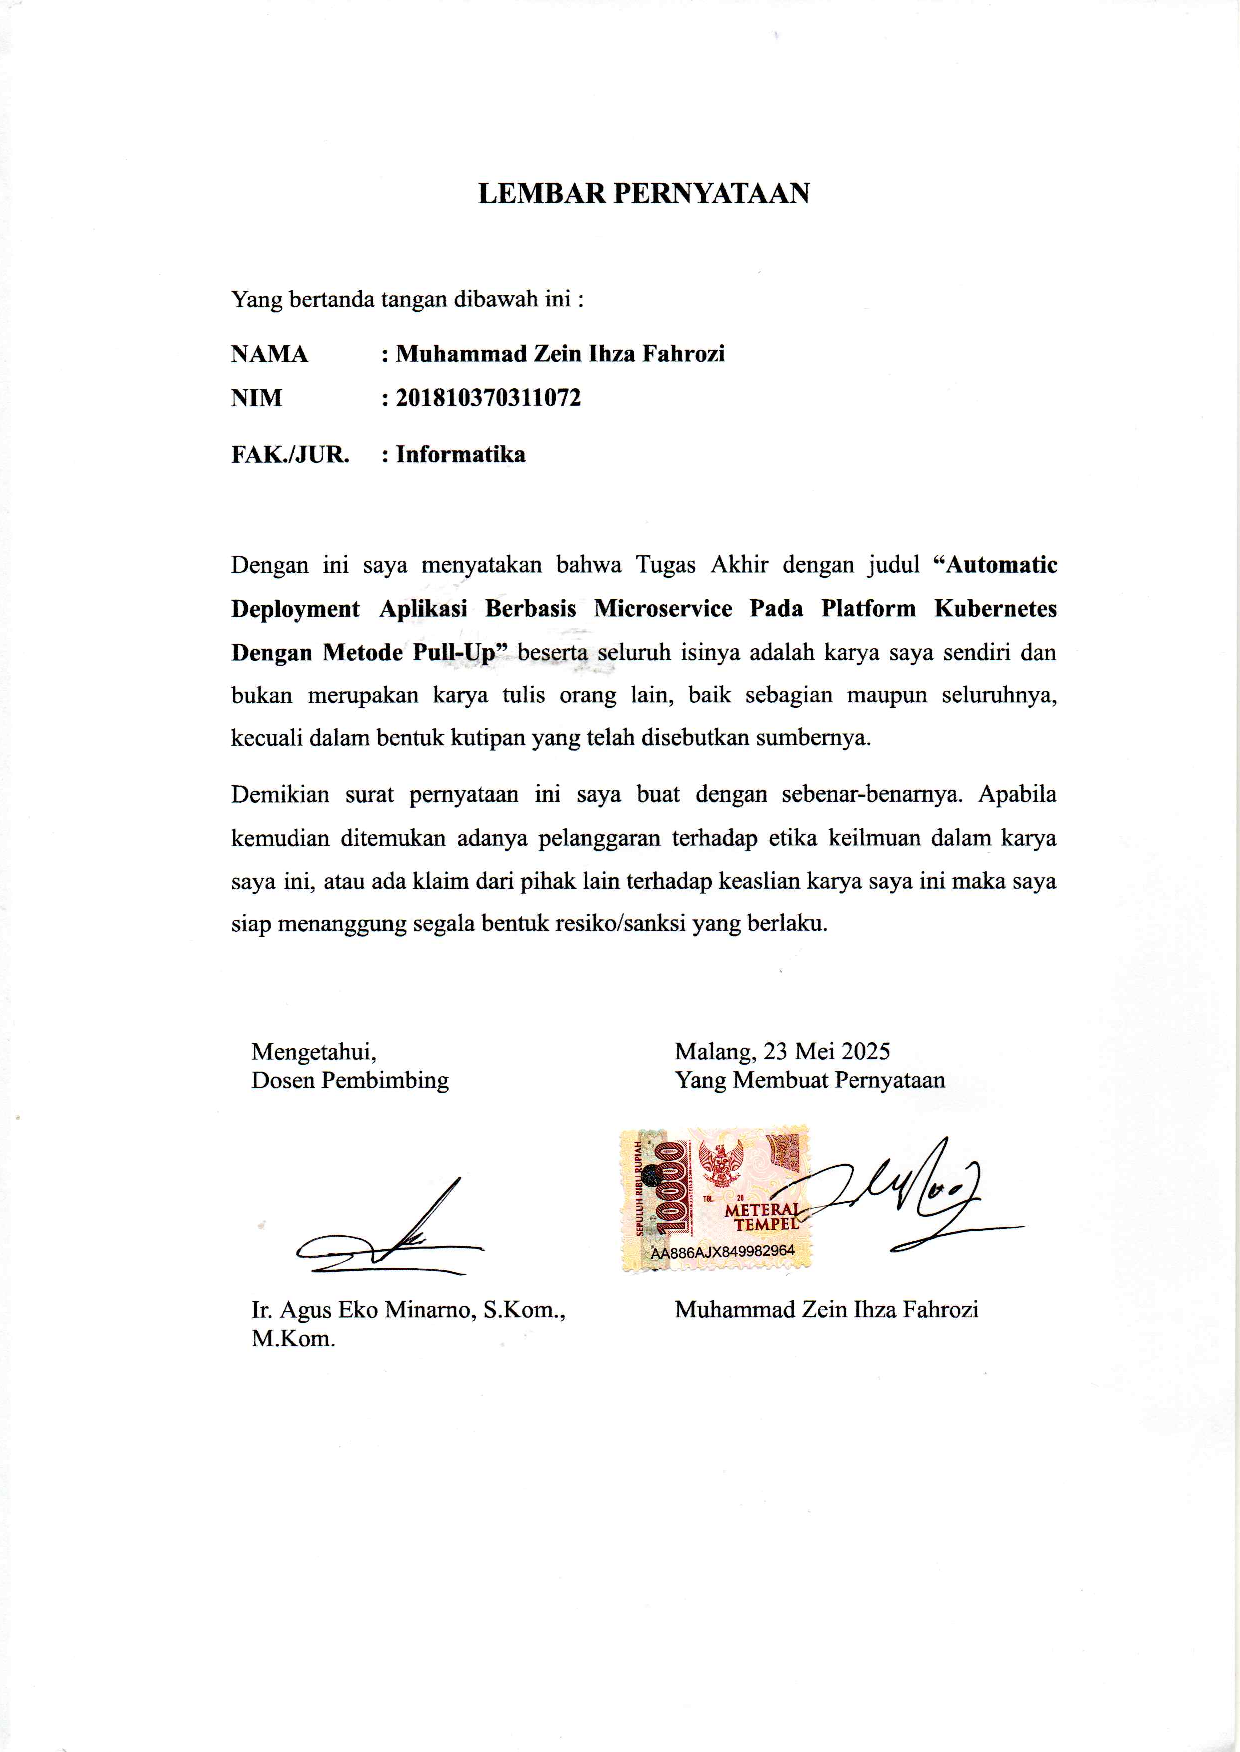
\includegraphics[width=\textwidth,page=1]{misc/lembar-pernyataan-scan.pdf}
\end{center}

\newpage


% Abstrak
%
% Halaman Abstract
\phantomsection \addcontentsline{toc}{chapter}{ABSTRAK}
\chapter*{ABSTRAK}

\begin{singlespace}
	\blindtext \\[20pt]
	Keywords: \textit{Information System, Testing Project}
\end{singlespace}

\newpage

\phantomsection \addcontentsline{toc}{chapter}{ABSTRACT}
\chapter*{ABSTRACT}

\begin{singlespace}
	\blindtext \\[20pt]
	Keywords: \textit{Information System, Testing Project}
\end{singlespace}

\newpage


% Lembar Persembahan
\phantomsection \addcontentsline{toc}{chapter}{LEMBAR PERSEMBAHAN}
\chapter*{\uppercase{LEMBAR PERSEMBAHAN}}
\vspace{1cm}

\begin{center}
    ``To Be Added Bismillah''
\end{center}

\newpage


% Daftar Isi
\vspace*{-2.5cm}
\tableofcontents
\phantomsection \addcontentsline{toc}{chapter}{DAFTAR ISI}
\clearpage
% Daftar Tabel
\vspace*{-2.5cm}
\listoftables
\phantomsection \addcontentsline{toc}{chapter}{DAFTAR TABEL}
\clearpage
% Daftar Gambar
\vspace*{-2.5cm}
\listoffigures
\phantomsection
\addcontentsline{toc}{chapter}{DAFTAR GAMBAR}
\clearpage




% Merubah Nama Bibliografi ke Daftar Pustaka

% %%%%%%%%%%%%%%%%%%%%%%%%%%%%%%%%%%%%%%%%%%%%%%%%%%%%%%%%%%
% DAFTAR PUSTAKA
% %%%%%%%%%%%%%%%%%%%%%%%%%%%%%%%%%%%%%%%%%%%%%%%%%%%%%%%%%%
\renewcommand{\bibname}{DAFTAR PUSTAKA}
\phantomsection
\addcontentsline{toc}{chapter}{DAFTAR PUSTAKA}
% Daftar Pustaka
\bibliographystyle{IEEEtranN}
\bibliography{references}

\end{document}